\documentclass{oblivoir}
%%%Default packages
\usepackage{amsmath,amssymb,amsthm,kotex,tabu,graphicx,pifont}
\usepackage{../kswrapfig}

\usepackage{gensymb} %\degree

%%%More packages
%\usepackage{caption,subcaption}
%\usepackage[perpage]{footmisc}
%
\usepackage[skipabove=10pt,innertopmargin=10pt,nobreak=true]{mdframed}

\usepackage[inline]{enumitem}
\setlist[enumerate,1]{label=(\arabic*)}
\setlist[enumerate,2]{label=(\alph*)}

\usepackage{multicol}
\setlength{\columnsep}{30pt}
\setlength{\columnseprule}{1pt}
%
%\usepackage{forest}
%\usetikzlibrary{shapes.geometric,arrows.meta,calc}
%
%%%defi theo exam prob rema proo
%이 환경들 아래에 문단을 쓸 경우 살짝 들여쓰기가 되므로 \hspace{-.7em}가 필요할 수 있다.

\newcounter{num}
\newcommand{\defi}[1]
{\noindent\refstepcounter{num}\textbf{정의 \arabic{num})} #1\par\noindent}
\newcommand{\theo}[1]
{\noindent\refstepcounter{num}\textbf{정리 \arabic{num})} #1\par\noindent}
\newcommand{\revi}[1]
{\noindent\refstepcounter{num}\textbf{복습 \arabic{num})} #1\par\noindent}
\newcommand{\exam}[1]
{\bigskip\bigskip\noindent\refstepcounter{num}\textbf{예시 \arabic{num})} #1\par\noindent}
\newcommand{\prob}[1]
{\bigskip\bigskip\noindent\refstepcounter{num}\textbf{문제 \arabic{num})} #1\par\noindent}
\newcommand{\rema}[1]
{\bigskip\bigskip\noindent\refstepcounter{num}\textbf{참고 \arabic{num})} #1\par\noindent}
\newcommand{\proo}
{\bigskip\noindent\textsf{증명)}}

\newenvironment{talign}
 {\let\displaystyle\textstyle\align}
 {\endalign}
\newenvironment{talign*}
 {\let\displaystyle\textstyle\csname align*\endcsname}
 {\endalign}
%
%%%Commands

\newcommand{\procedure}[1]{\begin{mdframed}\vspace{#1\textheight}\end{mdframed}}

\newcommand\an[1]{\par\bigskip\noindent\textbf{문제 \ref{#1})}\par\noindent}

\newcommand\ann[2]{\par\bigskip\noindent\textbf{문제 \ref{#1})}\:\:#2\par\medskip\noindent}

\newcommand\ans[1]{\begin{flushright}\textbf{답 : }#1\end{flushright}}

\newcommand\anssec[1]{\bigskip\bigskip\noindent{\large\bfseries#1}}

\newcommand{\pb}[1]%\Phantom + fBox
{\fbox{\phantom{\ensuremath{#1}}}}

\newcommand\ba{\,|\,}

\newcommand\ovv[1]{\ensuremath{\overline{#1}}}
\newcommand\ov[2]{\ensuremath{\overline{#1#2}}}
%
%%%% Settings
%\let\oldsection\section
%
%\renewcommand\section{\clearpage\oldsection}
%
%\let\emph\textsf
%
%\renewcommand{\arraystretch}{1.5}
%
%%%% Footnotes
%\makeatletter
%\def\@fnsymbol#1{\ensuremath{\ifcase#1\or
%*\or **\or ***\or
%\star\or\star\star\or\star\star\star\or
%\dagger\or\dagger\dagger\or\dagger\dagger\dagger
%\else\@ctrerr\fi}}
%
%\renewcommand{\thefootnote}{\fnsymbol{footnote}}
%\makeatother
%
%\makeatletter
%\AtBeginEnvironment{mdframed}{%
%\def\@fnsymbol#1{\ensuremath{\ifcase#1\or
%*\or **\or ***\or
%\star\or\star\star\or\star\star\star\or
%\dagger\or\dagger\dagger\or\dagger\dagger\dagger
%\else\@ctrerr\fi}}%
%}   
%\renewcommand\thempfootnote{\fnsymbol{mpfootnote}}
%\makeatother
%
%%% 객관식 선지
\newcommand\one{\ding{172}}
\newcommand\two{\ding{173}}
\newcommand\three{\ding{174}}
\newcommand\four{\ding{175}}
\newcommand\five{\ding{176}}
\usepackage{tabto,pifont}
%\TabPositions{0.2\textwidth,0.4\textwidth,0.6\textwidth,0.8\textwidth}

\newcommand\taba[5]{\par\noindent
\one\:{#1}
\tabto{0.2\textwidth}\two\:\:{#2}
\tabto{0.4\textwidth}\three\:\:{#3}
\tabto{0.6\textwidth}\four\:\:{#4}
\tabto{0.8\textwidth}\five\:\:{#5}}

\newcommand\tabb[5]{\par\noindent
\one\:{#1}
\tabto{0.33\textwidth}\two\:\:{#2}
\tabto{0.67\textwidth}\three\:\:{#3}\medskip\par\noindent
\four\:\:{#4}
\tabto{0.33\textwidth}\five\:\:{#5}}

\newcommand\tabc[5]{\par\noindent
\one\:{#1}
\tabto{0.5\textwidth}\two\:\:{#2}\medskip\par\noindent
\three\:\:{#3}
\tabto{0.5\textwidth}\four\:\:{#4}\medskip\par\noindent
\five\:\:{#5}}

\newcommand\tabd[5]{\par\noindent
\one\:{#1}\medskip\par\noindent
\two\:\:{#2}\medskip\par\noindent
\three\:\:{#3}\medskip\par\noindent
\four\:\:{#4}\medskip\par\noindent
\five\:\:{#5}}
%
%%%% fonts
%
%\usepackage{fontspec, xunicode, xltxtra}
%\setmainfont[]{은 바탕}
%\setsansfont[]{은 돋움}
%\setmonofont[]{은 바탕}
%\XeTeXlinebreaklocale "ko"
%%%%
\begin{document}

\title{수학(하) : 09 명제}
\author{}
\date{\today}
\maketitle
\tableofcontents
\newpage

%%proposition
\section{명제와 조건, 진리집합}

%
\exam{}
\begin{enumerate}\label{proposition1}
\item
`참과 거짓을 분명하게 판별할 수 있는 문장이나 식’을 \fbox{명제}라고 한다.
\begin{quote}
\(p_1\) : 산화반응이 일어나면 열이 발생한다.\\
\(p_2\) : \(9\)는 \(3\)의 배수이다.\\
\(p_2\) : \(4\times3\le9\)\\
\(p_3\) : 서울에서 전주까지는 멀다.\\
\(p_4\) : 연근조림은 맛있는 음식이다.
\end{quote}
에서 \(p_1\)과 \(p_2\)는 참이고 \(p_3\)는 거짓이다.
따라서 \(p_1\), \(p_2\), \(p_3\)는 명제이다.
하지만 \(p_4\)와 \(p_5\)는 참인지 거짓인지 판단할 수 없으므로 명제가 아니다.
\item
한편
\begin{quote}
\(p\) : \(x\)는 \(4\)의 약수이다.\\
\(q\) : \(x^2-7x+10=0\)
\end{quote}
와 같이 미지수 \(x\)가 포함된 경우,  \(x\)의 값에 따라 참이 될 수도 있고 거짓이 될 수도 있다.\footnotemark
\footnotetext{
\raisebox{-.5\height}{\begin{tabular}{c@{\quad}l}
\(p\)의 경우,	&\(x=1\)이면 참이다.\\
			&\(x=2\)이면 참이다.\\
			&\(x=3\)이면 거짓이다.
\end{tabular}}
\raisebox{-.5\height}{\begin{tabular}{c@{\quad}l}
\(q\)의 경우,	&\(x=1\)이면 거짓이다.\\
			&\(x=2\)이면 참이다.\\
			&\(x=3\)이면 거짓이다.
\end{tabular}}
}
따라서 명제는 아니다.
이처럼 미지수가 포함된 문장이나 식은 \fbox{조건}이라고 부른다.
\item
조건 \(p\)를 만족시키는 \(x\)의 값에는 \(1\), \(2\), \(4\)가 있다.
이것들로 이루어진 집합 \[P=\{1,2,4\}\]를 \(p\)의 \fbox{진리집합}이라고 부른다.
마찬가지로
\[Q=\left\{2,5\right\}\]
이다.
\newpage
\item
\(x\)가 실수일 때, 두 조건 \(r\), \(s\)를
\begin{quote}
\(r\) : \(x^2\ge0\)\\
\(s\) : \(|x|+1=0\)
\end{quote}
이라고 하자.
\(r\)은 항상 성립하므로
\[R=U\]
이다.
또 \(s\)는 절대 성립할 수 없으므로
\[S=\varnothing\]
\end{enumerate}
%
%%
%\exam{}
%\(x\)가 실수일 때, 다음 조건들의 진리집합을 나타내어라.\\
%(단, \(\varnothing\)은 공집합, \(U\)는 전체집합을 나타낸다.)
%\begin{quote}
%\(p\) : \(x\)는 \(4\)로 나누었을 때 나머지가 \(1\)인 수\\
%\(q\) : \(|x-3|<2\)\\
%\(r\) : \(x^2\ge0\)
%\end{quote}
%\begin{mdframed}
%\(p\)를 그대로 사용하여
%\[P=\{x\ba\text{\(x\)는 \(4\)로 나누었을 때 나머지가 \(1\)인 수}\}\]
%로 표현할 수 있다.
%한편, \(p\)를만족시키려면 \(x=4k-3\)이므로(단, \(k\)는 자연수)
%\[P=\{4k-3\ba\text{\(k\)는 자연수}\}\]
%로 표현해도 된다.
%\(q\)의 부등식을 풀면 \(-2<x-3<2\), \(1<x<5\)이므로
%\[Q=\{x\ba1<x<5\}\]
%이다.
%\(r\)의 경우, \(x\)가 어떤 실수이건 성립하므로
%\[R=U\]
%\end{mdframed}

%
\prob{}\label{proposition2}
다음 중 명제의 개수를 \(a\), 참인 명제의 개수를 \(b\), 조건의 개수를 \(c\)라고 할 때, \(a+b+c\)의 값을 구하여라.
\begin{quote}
\(p_1\) : 염산의 pH는 7보다 크다.\\
\(p_2\) : 삼각김밥은 맛있다.\\
\(p_3\) : 이등변삼각형의 두 변의 길이는 같다.\\
\(p_4\) : 세 변의 길이가 \(3\), \(5\), \(6\)인 삼각형은 예각삼각형이다.\\
\(p_5\) : \(4+7>10\)\\
\(p_6\) : \(4+x>10\)\\
\(p_7\) : 모든 순환소수는 유리수이다.\\
\end{quote}

%
\prob{}\label{proposition3}
\(x\)가 실수일 때, 다음 조건들의 진리집합을 구하여라.
\begin{quote}
\(p\) : \(x\)는 \(4\)의 배수이다.\\
\(q\) : \(x^3-6x^2+8x=0\)\\
\(r\) : \(x^2-4x+4\le0\)\\
\(s\) : \(x^2-4x+4\ge0\)
\end{quote}

%%negation
\section{부정}
%
\exam{명제의 부정}\label{negation1}
명제 \(p\)의 부정은 \(\sim p\)로 표현한다.%
\footnote{읽을 때는 `not \(p\)’라고 읽는다.}
만약
\begin{quote}
\(p\) : \(2\)는 \(4\)의 약수이다.
\end{quote}
이면 \(p\)의 부정은
\begin{quote}
\(\sim p\) : \(2\)는 \(4\)의 약수가 아니다.
\end{quote}
이다.
%또,
%\begin{quote}
%\(p\) : \(2+5<0\)
%\end{quote}
%이면 \(p\)의 부정은
%\begin{quote}
%\(\sim p\) : \(2+5\le0\)
%\end{quote}
%이다.

\begin{mdframed}
%
\theo{}\label{negation2}
명제 \(p\)에 대해
\begin{itemize}
\item
\(p\)가 참이면 \(\sim p\)는 거짓이다
\item
\(p\)가 거짓이면 \(\sim p\)는 참이다.
\end{itemize}
\end{mdframed}

%
\exam{조건의 부정}\label{negation3}
\par\noindent
\begin{minipage}{0.5\textwidth}
\(U=\{1,2,3,4,5\}\)일 때,
\begin{quote}
\(p\) : \(x<3\)
\end{quote}
이면 \(P=\{1,2\}\)이다.
\(p\)의 부정은
\begin{quote}
\(\sim p\) : \(x\ge3\)
\end{quote}
이고 \(\sim p\)의 진리집합은 \(\{3,4,5\}\)인데\\
이것은 \(P^c\)이다.
\end{minipage}
\begin{minipage}{0.45\textwidth}
\begin{center}
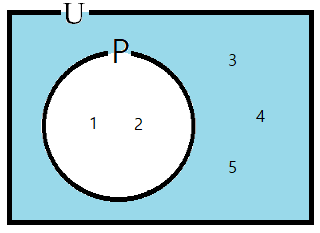
\includegraphics[width=0.66\textwidth]{negation_3}
\end{center}
\end{minipage}

\begin{mdframed}
%
\theo{}\label{negation_4}
조건 \(p\)에 대해
\begin{itemize}
\item
\(\sim p\)의 진리집합은 \(P^c\)이다.
\end{itemize}
\end{mdframed}

%
\subsection{“또는”과 “그리고”의 부정}
%
\exam{\(U=\{1,2,3,4,5,6\}\)일 때, 두 조건 \(p\), \(q\)를}\label{negation5}
%\noindent
%\begin{minipage}{0.65\textwidth}
%(1)\:\:\(U=\{1,2,3,4,5,6\}\)일 때,
%\begin{quote}
%\(p\) : \(x\)는 \(4\)의 약수이다.\\
%\(q\) : \(x\)는 \(6\)의 약수이다.
%\end{quote}
%라고 하자.
%\end{minipage}
%\begin{minipage}{0.3\textwidth}
%\begin{center}
%\includegraphics[width=\textwidth]{negation_4-1}
%\end{center}
%\end{minipage}
%
%%
%\noindent
%\begin{minipage}{0.65\textwidth}
%(2)\:\:새로운 조건
%\begin{quote}
%\(p\) 또는 \(q\) : 
%\(x\)는 \(4\)의 약수이거나 \(6\)의 약수이다.
%\end{quote}
%의 진리집합은
%\[P\cup Q\]
%이다.
%\end{minipage}
%\begin{minipage}{0.3\textwidth}
%\begin{center}
%\includegraphics[width=\textwidth]{negation_4-2}
%\end{center}
%\end{minipage}
%
%%
%\noindent
%\begin{minipage}{0.65\textwidth}
%(3)\:\:또한
%\begin{quote}
%\(p\) 그리고 \(q\) : 
%\(x\)는 \(4\)의 약수이고 \(6\)의 약수이다.
%\end{quote}
%의 진리집합은
%\[P\cap Q\]
%이다.
%\end{minipage}
%\begin{minipage}{0.3\textwidth}
%\begin{center}
%\includegraphics[width=\textwidth]{negation_4-3}
%\end{center}
%\end{minipage}
%
%%
%\noindent
%\begin{minipage}{0.65\textwidth}
%(4)\:\:\(p\) 또는 \(q\)의 부정은 진리집합이 \((P\cup Q)^c\)이다.
%즉 \(P^c\cup Q^c\)이다.
%따라서
%\begin{quote}
%\(\sim(p\text{ 그리고 }q)\) : 
%\(x\)는 \(4\)의 약수가 아니고 \(6\)의 약수도 아니다.
%\end{quote}
%\end{minipage}
%\begin{minipage}{0.3\textwidth}
%\begin{center}
%\includegraphics[width=\textwidth]{negation_4-4}
%\end{center}
%\end{minipage}
%\noindent
\begin{minipage}{0.65\textwidth}
\begin{quote}
\(p\) : \(x\)는 \(4\)의 약수이다.\\
\(q\) : \(x\)는 \(6\)의 약수이다.
\end{quote}
라고 하자.
\end{minipage}
\begin{minipage}{0.3\textwidth}
\begin{center}
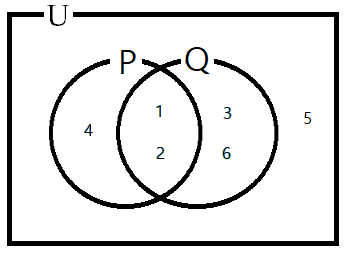
\includegraphics[width=\textwidth]{negation_5-1}
\end{center}
\end{minipage}

\medskip
두 조건 \(p\), \(q\)로 만든 네 명제
\begin{quote}
\(p\) 또는 \(q\) 				\tabto{0.25\textwidth}: \(x\)는 \(4\)의 약수이거나 \(6\)의 약수이다.\\
\(p\) 그리고 \(q\) 			\tabto{0.25\textwidth}: \(x\)는 \(4\)의 약수이고 \(6\)의 약수이다.\\
\(\sim p\) 또는 \(\sim q\)		\tabto{0.25\textwidth}: \(x\)는 \(4\)의 약수가 아니거나 \(6\)의 약수가 아니다.\\
\(\sim p\) 그리고 \(\sim q\)	\tabto{0.25\textwidth}: \(x\)는 \(4\)의 약수가 아니고 \(6\)의 약수도 아니다.
\end{quote}
를 생각하자.

\medskip
`\(p\) 또는 \(q\)’의 부정은 진리집합이
\[(P\cup Q)^c\]
이다.
그런데 이것은 `\(\sim p\) 그리고 \(\sim q\)’의 진리집합인
\[P^c\cap Q^c\]
와 같다(드 모르간의 법칙).
따라서
%\fbox{\(\sim(p\text{ 또는 }q)\iff\sim p\text{ 그리고 }\sim q\)}
%\fbox{\(p\text{ 또는 }q\)}의 부정은 \fbox{\(\sim p\) 그리고 \(\sim q\)}이다.
%마찬가지로 생각하면
%\fbox{\(p\text{ 그리고 }q\)}의 부정은 \fbox{\(\sim p\) 또는 \(\sim q\)}이다.
\begin{center}
\fbox{\(p\text{ 또는 }q\)}의 부정은 \fbox{\(\sim p\) 그리고 \(\sim q\)}이다.
\end{center}
마찬가지로 생각하면
\begin{center}
\fbox{\(p\text{ 그리고 }q\)}의 부정은 \fbox{\(\sim p\) 또는 \(\sim q\)}이다.
\end{center}
\begin{mdframed}

%
\theo{}
\begin{itemize}\label{negation6}
\item
\(\sim(p\text{ 또는 }q)\iff\sim p\text{ 그리고 }\sim q\)
\item
\(\sim(p\text{ 그리고 }q)\iff\sim p\text{ 또는 }\sim q\)
\end{itemize}
\end{mdframed}

%
\prob{다음 중 옳은 것을 고르시오.}\label{negation7}
\vspace{-20pt}
\tabd
{삼각형 \(ABC\)는 예각삼각형이다. \tabto{0.47\textwidth}\(\xrightarrow{\text{부정}}\) 삼각형 \(ABC\)는 둔각삼각형이다.}
%{사각형 \(ABCD\)는 직사각형이다. \tabto{0.47\textwidth}\(\xrightarrow{\text{부정}}\) 사각형 \(ABCD\)는 마름모이다.}
{\(x\)는 \(9\)의 약수이다. 	\tabto{0.47\textwidth}\(\xrightarrow{\text{부정}}\) \(x\)는 \(9\)의 배수이다.}
{\(x<3\) 					\tabto{0.47\textwidth}\(\xrightarrow{\text{부정}}\) \(x>3\)}
{\(x=1\) 또는 \(x=3\)이다. 	\tabto{0.47\textwidth}\(\xrightarrow{\text{부정}}\)  \(x\neq1\) 또는 \(x\neq 3\)이다.}
{\(x\le1\) 또는 \(x\ge 3\)이다. 	\tabto{0.47\textwidth}\(\xrightarrow{\text{부정}}\) \(x>1\)이고 \(x<3\)이다.}

%
\prob{다음 명제의 부정을 말하고, 그것의 참, 거짓을 판별하시오.}\label{negation8}
\begin{enumerate*}[itemjoin={\qquad\qquad}]
\item
\(\sqrt{25}\)는 무리수이다.
\item
\(11\)은 짝수이거나 \(3\)의 배수이다.
\end{enumerate*}

%
\prob{}\label{negation9}
전체집합 \(U=\{0,1,2,3,4,5\}\)에서 두 조건
\[p:x\ge2,\qquad\qquad q:x^2+x-6=0\]
의 진리집합을 각각 \(P\), \(Q\)라고 할 때, 집합 \(P\), \(Q\) 사이의 포함관계를 나타내시오.

%
\prob{}\label{negation10}
조건 `\(2<x<5\)’의 부정을 말하여라.

%%
%\prob{}
%\(U=\{x\ba x\text{는 \(10\) 이하의 자연수}\}\)이고
%\begin{quote}
%\(p\) : \(x\ge5\)\\
%\(q\) : \(x\le5\)\\
%\(r\) : \(x\)는 소수
%\end{quote}
%일 때,

\newpage
%
\subsection{“모든”과 “어떤”의 부정}
\vspace{-20pt}
%
\exam{다음 명제들에 대해 생각해보자.}
\begin{quote}\label{negation11}
\(p\) : 모든 자연수 \(x\)에 대하여 \(x>0\)이다.\footnotemark\\
\(q\) : 모든 자연수 \(x\)에 대하여 \(x>3\)이다.
\end{quote}
\footnotetext{
\parbox[t]{0.45\textwidth}{
임의의 자연수 \(x\)에 대하여 \(x>0\)이다.\\
\(x\)가 자연수이면 \(x>0\)이다.\\
자연수 \(x\)의 값에 관계없이 \(x>0\)이다.}
%\end{tabular}
%\begin{tabular}{l}
%임의의 자연수 \(x\)에 대하여 \(x>0\)이다.\\
%\(x\)가 자연수이면 \(x>0\)이다.
%\end{tabular}
등으로 표현되기도 한다.
}
\(p\)는 참이다.
모든 자연수는 \(0\)보다 크기 때문이다.
하지만 \(q\)는 거짓이다.\\
\(3\)보다 크지 않은 자연수도 있기 때문이다.
\begin{quote}
\(r\) : 어떤 자연수 \(x\)에 대하여 \(x^2=9\)이다.\footnotemark\\
\(s\) : 어떤 자연수 \(x\)에 대하여 \(x^2=3\)이다.
\end{quote}
\footnotetext{
\parbox[t]{0.55\textwidth}{
%\begin{tabular}{l}
\(x^2=9\)를 만족시키는 자연수 \(x\)가 존재한다.\\
적어도 한 개 이상의 자연수 \(x\)에 대해 \(x^2=9\)이다.}
%\end{tabular}
등으로 표현되기도 한다.
}
\(r\)은 참이다.
\(x=3\)이면 \(x^2=9\)를 만족시키기 때문이다.
하지만 \(s\)는 거짓이다.
자연수 중에서는 \(x^2=3\)을 만족시키는 수가 없기 때문이다.

\bigskip
이처럼 조건 \(p(x)\)에 대하여,% `모든’이나 `어떤’을 포함시켜
\begin{center}
\fbox{모든 \(x\)에 대하여 \(p(x)\)이다.}\qquad\fbox{어떤 \(x\)에 대하여 \(p(x)\)이다.}
\end{center}
와 같은 명제를 만들 수 있다.
%이 명제들은 각각
%\begin{center}
%\fbox{임의의 \(x\)에 대하여 \(p(x)\)이다.}\qquad\fbox{\(p(x)\)를 만족시키는 \(x\)가 존재한다.}
%%\fbox{모든 \(x\)에 대하여 \(p(x)\)이다.}\qquad\fbox{어떤 \(x\)에 대하여 \(p(x)\)이다.}
%\end{center}
%라고 표현되기도 한다.
%\footnote{각각 \fbox{\(\forall x,\:\: p(x)\)}, \fbox{\(\exists x,\:\: p(x)\)}로 표현하기도 한다.
%$\forall$은 `for all’에서의 a의 대문자 A를 뒤집은 기호로 `전칭양화사’라고 불린다.
%$\exists$는 `exist’에서의 e의 대문자 E를 뒤집은 기호로 `존재양화사’라고 불린다.
%}

%
\prob{다음 명제의 참, 거짓을 판별하시오.}
\begin{enumerate}\label{negation12}\tightlist
\item
모든 실수 \(x\)에 대하여 \(x^2+1>0\)이다.
\item
어떤 자연수 \(x\)에 대하여 \(x<1\)이다.
\item
모든 실수 \(x\)에 대하여 \((x+2)^2-1>0\)이다.
\item
어떤 실수 \(x\)에 대하여 \(x(x-1)=0\)이다.
\end{enumerate}

\vspace{-10pt}
%
\prob{다음 명제의 참, 거짓을 판별하시오.}
\begin{enumerate}\label{negation13}\tightlist
\item
모든 소수는 홀수이다.
\item
모든 직사각형은 사다리꼴이다.
\item
어떤 이등변삼각형은 정삼각형이다.
\item
어떤 홀수는 \(24\)의 약수이다.
\end{enumerate}

%\newpage
%
\exam{세 학생 \(A\), \(B\), \(C\)에 대해, 다음 명제들을 생각하자.\footnotemark}
\begin{quote}\label{negation14}
\(p\) : 모든 학생은 남자이다.\\
\(q\) : 어떤 학생은 남자이다.\\
\(r\) : 모든 학생은 여자이다.\\
\(s\) : 어떤 학생은 여자이다.
\end{quote}
%발생할 수 있는 경우는 오른쪽에 나타난 8가지이다.
예를 들어
\begin{itemize}
\item[①]
셋 다 남자이면,\\
\(p\)는 참이고, \(q\)도 참이다.
하지만 \(r\)은 거짓이고 \(s\)도 거짓이다.
\item[②]
\(A\), \(B\)는 남자, \(C\)는 여자이면,\\
\(p\)는 거짓이고, \(q\)는 참이다.
또 \(r\)은 거짓이고 \(s\)는 참이다.
\end{itemize}
발생할 수 있는 모든 경우를 아래에 표현해보면
\begin{center}
\begin{tabu}[tabulinesep=100pt]{c|ccc|cccc}
	&\(A\)	&\(B\)	&\(C\)	&\(p\)	&\(q\)	&\(r\)	&\(s\)\\\hline
①	&남		&남		&남		&참		&참		&거짓	&거짓\\
②	&남		&남		&여		&거짓	&참		&거짓	&참	\\
③	&남		&여		&남\\
④	&남		&여		&여\\
⑤	&여		&남		&남\\
⑥	&여		&남		&여\\
⑦	&여		&여		&남\\
⑧	&여		&여		&여
\end{tabu}
\end{center}
이다.
(빈 칸을 모두 채워보자.)
\footnotetext{모든 학생은 남자 아니면 여자라고 가정하자.}

\newpage
정리하면,
\begin{itemize}
\item
\(p\)는 ①이면 참이고 ②\(\sim\)⑧이면 거짓이다.
\item
\(q\)는 ①\(\sim\)⑦이면 참이고 ⑧이면 거짓이다.
\item
\(r\)는 ①\(\sim\)⑦이면 거짓이고 ⑧이면 참이다.
\item
\(s\)는 ①이면 거짓이고 ②\(\sim\)⑧이면 참이다.
\end{itemize}
따라서 \(p\)의 부정은 \(s\)이다.
또 \(q\)의 부정은 \(r\)이다.

\begin{center}
\fbox{모든 학생은 남자이다}의 부정은 \fbox{어떤 학생은 여자이다}
\end{center}
\begin{center}
\fbox{어떤 학생은 남자이다}의 부정은 \fbox{모든 학생은 여자이다}
\end{center}
\(x\)를 \(A\), \(B\), \(C\) 중에 하나라고 하고, \(p(x)\)를
\[p(x)\::\:x\text{는 남자이다.}\]
라고 하면 다음과 같이 쓸 수도 있다.
\begin{center}
\fbox{모든 \(x\)에 대해 \(p(x)\)이다}의 부정은 \fbox{어떤 \(x\)에 대해 \(\sim p(x)\)이다}\\
\end{center}
\begin{center}
\fbox{어떤 \(x\)에 대해 \(p(x)\)이다}의 부정은 \fbox{모든 \(x\)에 대해 \(\sim p(x)\)이다}\\
\end{center}

%\end{minipage}
%\begin{minipage}{0.25\textwidth}
%\end{minipage}

%명제 (1)의 부정이 무엇인지 한번 생각해보자.
%`모든 학생은 남자이다'의 부정이니 `모든 학생은 여자이다'라고 답하기 쉽지만 실제로 그렇지 않다.
%
%세 학생의 성별의 가능한 경우를 모두 나열해보면 오른쪽 그림과 같은데, 명제 (1)이 성립하는 경우의 반대는 명제 (4)이다.
%따라서 명제 (1)의 부정은 (4)이다.
%즉
%\begin{center}
%\fbox{모든 학생은 남자이다.}
%\end{center}
%의 부정은
%\begin{center}
%\fbox{어떤 학생은 남자가 아니다.}
%\end{center}
%이다.


\begin{mdframed}
%
\theo{}
\begin{itemize}\label{negation15}
\item
\(\sim\left(\text{모든 \(x\)에 대하여 \(p(x)\)이다.}\right)\iff\text{어떤 \(x\)에 대하여 \(\sim p(x)\)이다.}\)
\item
\(\sim\left(\text{어떤 \(x\)에 대하여 \(p(x)\)이다.}\right)\iff\text{모든 \(x\)에 대하여 \(\sim p(x)\)이다.}\)
\end{itemize}
\end{mdframed}

%
\prob{다음 명제의 부정을 말하고, 그것의 참, 거짓을 판별하시오.}
\begin{enumerate}\label{negation16}
\item
모든 실수 \(x\)에 대하여 \(x^2>0\)이다.
\item
어떤 실수 \(x\)에 대하여 \(x^2=10\)이다.
\end{enumerate}


%%
\section{\(p\to q\) 꼴의 명제}

%
\exam{}
\begin{enumerate}\label{pq1}
\item
%두 조건 \(p\), \(q\)에 대하여 \fbox{\(p\)이면 \(q\)이다}꼴의 명제가 있다.\\
%이때 \(p\)를 `가정’, \(q\)를 `결론’이라고 부른다.
두 조건 \(p\), \(q\)에 대하여 `\(p\)이면 \(q\)이다’꼴의 명제가 있다.\\
이때 \(p\)를 \fbox{가정}, \(q\)를 \fbox{결론}이라고 부른다.
예를 들어
\begin{quote}
봄이 오면 꽃이 핀다.
\end{quote}
에서의 가정은 `봄이 온다’이고 결론은 `꽃이 핀다’이다.
또
\begin{quote}
\(n\)이 \(4\)의 약수이면 \(n\)은 \(8\)의 약수이다.
\end{quote}
에서의 가정은 `\(n\)이 \(4\)의 약수이다.’이고 결론은 `\(n\)이 \(8\)의 약수이다.’이다.
\item
위의 명제
\begin{quote}
\(n\)이 \(4\)의 약수이면 \(n\)은 \(8\)의 약수이다.
\end{quote}
은 참이다.
가정 \(p\)와 결론 \(q\)의 진리집합을 각각 \(P\), \(Q\)라고 하면,
\[P=\{1,2,4\},\quad Q=\{1,2,4,8\}\]
이다.
즉 \(P\subset Q\)가 성립한다.
\item
하지만
\begin{quote}
\(n\)이 \(4\)의 약수이면 \(n\)은 \(6\)의 약수이다.
\end{quote}
는 거짓이다.
이 경우
\[P=\{1,2,4\},\quad Q=\{1,2,3,6\}\]
이므로 \(P\not\subset Q\)이다.
이 명제가 거짓인 이유는 \(n=4\)인 경우가 있기 때문이다.
%, 즉 \(P\subset Q\)가 성립하지 않는 이유는 \(n=4\)인 경우가 있기 때문이다.
이처럼, \(p\)는 만족시키지만 \(q\)는 만족시키지 않는 예를 \fbox{반례}라고 부른다.\footnotemark
\footnotetext{따라서 반례는 \(P\cap Q^c\)의 원소이다.}
\end{enumerate}

\begin{mdframed}
%
\theo{}
\begin{itemize}\label{pq2}
\item
\(P\subset Q\)이면 명제 \(p\to q\)는 참이다.
\item
\(P\not\subset Q\)이면 명제 \(p\to q\)는 거짓이다.%\footnote{이때, \(P\cap Q^c\)의 원소를 `반례’라고 부른다.}
\end{itemize}
\end{mdframed}

%
\exam{다음 명제의 참 거짓을 판별하고, 거짓인 경우 반례를 들어라.}
\begin{enumerate*}[itemjoin={,\qquad\qquad}]\label{pq3}
\item
\(x>5\)이면 \(x>3\)이다
\item
\(x^2=25\)이면 \(x=5\)이다
\end{enumerate*}
\begin{mdframed}
\begin{enumerate}
\item
\(P=\{x\ba x>5\},\:\: Q=\{x\ba x>3\}\)
이다.
따라서 \(P\subset Q\)가 성립하며 주어진 명제는 참이다.
\begin{center}
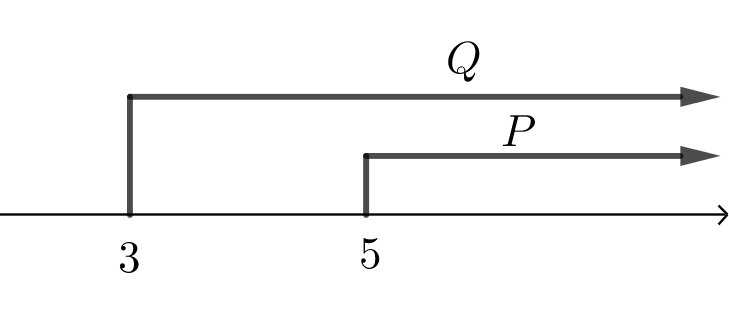
\includegraphics[width=0.4\textwidth]{pq_3}
\end{center}
\item
\(P=\{-5,5\},\:\: Q=\{5\}\)
이다.
따라서 \(P\subset Q\)가 성립하지 않으며 주어진 명제는 거짓이다.
이때 반례는 \(-5\)이다.
\end{enumerate}
\end{mdframed}
\ans{(1)\:참,\quad(2)\:거짓(반례 : \(-5\))}

%
\prob{다음 명제의 참 거짓을 판별하여라.}
\begin{enumerate}%[itemjoin={,\qquad\qquad}]
\label{pq4}
\item
\(2x-1=3\)이면 \(x^2-5x+6=0\)이다
\item
\(x^2+2x-3>0\)이면 \(x+1>0\)이다.
\end{enumerate}

%
\prob{다음 중에서 명제 `\(x\)와 \(y\)가 무리수이면 \(xy\)는 무리수이다.’의 반례가 될 수 있는 것은?}\label{pq5}
\vspace{-20pt}
\tabb
{\(x=1\), \(y=2\)}
{\(x=2\), \(y=\sqrt2\)}
{\(x=\sqrt3\), \(y=1\)}
{\(x=-\sqrt2\), \(y=\sqrt2\)}
{\(x=\sqrt2\), \(y=\sqrt2-1\)}
\newpage

%%
\subsection{역과 대우}
\begin{mdframed}
%
\defi{}\label{pq6}
주어진 명제 \(p\to q\)에서
\begin{itemize}
\item
명제 \(q\to p\)를 \(p\to q\)의 \fbox{역}이라고 한다.
\item
명제 \(\sim q\to\sim p\)를 \(p\to q\)의 \fbox{대우}이라고 한다.
\end{itemize}
\end{mdframed}

%
\exam{}
\begin{quote}\label{pq7}
\(n\)이 \(4\)의 약수이면 \(n\)은 \(8\)의 약수이다.
\end{quote}
의 역은
\begin{quote}
\(n\)이 \(8\)의 약수이면 \(n\)은 \(4\)의 약수이다.
\end{quote}
이고, 대우는
\begin{quote}
\(n\)이 \(8\)의 약수가 아니면 \(n\)은 \(4\)의 약수가 아니다.
\end{quote}
이다.

%
\prob{다음 명제의 역과 대우를 각각 말하고, 그것의 참, 거짓을 판별하시오.}
\begin{enumerate}\label{pq8}
\item
\(x^2-2x=0\)이면 \(x=2\)이다.
\item
\(x^2<16\)이면 \(-4<x<4\)이다.
\end{enumerate}

\bigskip
\(p\to q\)가 참이려면 \(P\subset Q\)이어야 하고, 
\(q\to p\)가 참이려면 \(Q\subset P\)이어야 하며, 
\(\sim q\to\sim p\)가 참이려면 \(Q^c\subset P^c\)이어야 한다.

\(P\subset Q\)인 것과 \(Q\subset P\)인 것은 서로 관련이 없지만, \(P\subset Q\)인 것과 \(Q^c\subset P^c\)는 완전히 같은 상태를 가리킨다.
따라서
\begin{mdframed}
%
\theo{}
\begin{itemize}\label{pq9}
\item
명제 \(p\to q\)가 참이라고 해서 그 역이 반드시 참인 것은 아니다.
\item
명제 \(p\to q\)가 참이면 그 대우도 참이다.
\item
명제 \(p\to q\)가 거짓이면 그 대우도 거짓이다.
\end{itemize}
\end{mdframed}

\newpage
%%
\subsection{필요조건과 충분조건}

\begin{mdframed}
%
\defi{}
\begin{enumerate}
\item
명제 \(p\to q\)가 참이면 \[p\Longrightarrow q\]로 나타낸다.
이때,
\begin{quote}
\(p\)는 \(q\)이기 위한 \fbox{충분조건}이다.
\end{quote}
\begin{quote}
\(q\)는 \(p\)이기 위한 \fbox{필요조건}이다.
\end{quote}
라고 말한다.
\item
명제 \(p\to q\)와 \(q\to p\)가 모두 참이면, 즉  \(p\Longrightarrow q\)이면서 \(q\Longrightarrow p\)이면
\[p\iff q\]로 나타낸다.
이때,
\begin{quote}
\(p\)는 \(q\)이기 위한 \fbox{필요충분조건}이다.\footnotemark
\end{quote}
라고 말한다.
\end{enumerate}
\end{mdframed}
\footnotetext{`\(p\)와 \(q\)가 동치이다.’ 라고도 말한다.}
%\(p\)와 \(q\)가 완전히 똑같은 말이라는 의미이다.}

%
\rema{}
%\begin{enumerate}
%\item
%두 조건
\begin{quote}
\(p\) : \(n\)은 \(4\)의 배수이다.\\
\(q\) : \(n\)은 짝수이다.
\end{quote}
에서 \(p\Longrightarrow q\)가 성립한다.
%반면 \(q\not\Longrightarrow p\)이기도 하다.
\begin{enumerate}
\item
\(p\)는 \(q\)이기 위한 충분조건이다.\\
%\(n\)이 \(4\)의 배수인 것은 \(n\)이 짝수이기 위한 충분조건이다.\\
\(n\)이 \(4\)의 배수인 것은 \(n\)이 짝수이기 위해서 이미 충분한 조건이기 때문이다.
%왜냐하면, \(n\)이 \(4\)의 배수이면 \(n\)은 이미(충분히) 짝수이기 때문이다.
\item
\(q\)는 \(p\)이기 위한 필요조건이다.\\
\(n\)은 짝수인 것은 \(n\)이 \(4\)의 배수가 되기 위해서 필요한 조건이기 때문이다.
%왜냐하면, \(n\)이 \(4\)의 배수가 되려면 \(n\)이 일단 짝수일 필요가 있기 때문이다.
%\item
%\(p\)는 \(q\)이기 위한 필요조건은 아니다.\\
%왜냐하면, \(n\)이 짝수라고 해서 \(n\)이 \(4\)의 배수일 필요는 없기 때문이다.
\end{enumerate}

%다음 명제를 생각하자.
%\begin{quote}
%\(n\)이 \(4\)의 배수이면 \(n\)은 짝수이다.
%\end{quote}
%이 명제는 참인 명제이다.
%아래 그림처럼 \(4\)의 배수들의 집합은 짝수들의 집합 안에 포함되기 때문이다.
%이때,
%\begin{quote}
%\fbox{\(n\)이 \(4\)의 배수이려면 일단 짝수일 \fbox{필요}가 있다.}
%\end{quote}
%
%\begin{quote}
%\fbox{만약 \(n\)이 \(4\)의 배수이면,  \(n\)은 이미 (충분히) 짝수이다.}
%\end{quote}
%\end{enumerate}


%%
\section{정의, 정리, 증명}
수학의 모든 논리체계는 정의와 정리, 증명으로 이루어져있다.
\begin{itemize}
\item
용어의 뜻을 명확하게 정한 문장을 \fbox{정의}라고 한다.
\item
참인 명제들 중 기본이 되는 명제들을 \fbox{정리}라고 한다.
\item
어떤 명제가 참임을 논리적으로 밝히는 과정을 \fbox{증명}이라고 한다.
\end{itemize}

%\bigskip

%
\prob{다음 중 정의와 정리를 구분하여라.}
\begin{enumerate}\label{proof1}
\item
이등변삼각형이란, 두 변의 길이가 같은 삼각형을 말한다.
\item
삼각형의 세 각의 크기의 합은 \(180^\circ\)이다.
%\item
%삼각형의 한 외각의 크기는 이웃하지 않은 두 내각의 크기의 합과 같다.
\item
\(a\neq0\)일 때, \(ax^2+bx+c=0\) 꼴의 방정식을 이차방정식이라고 한다.
%다항식 \(f(x)\), \(g(x)\)에 대해
%\(f(x)=g(x)Q(x)+R(x)\)
%를 만족시키고, \(R(x)\)의 차수가 \(f(x)\)의 차수보다 적으면 \(Q(x)\)를 몫, \(R(x)\)를 나머지라고 부른다.
%\item
%이차방정식 \(ax^2+bx+c=0\)의 근은 \(x=\frac{-b\pm\sqrt{b^2-4ac}}{2a}\)이다.
\item
이차방정식 \(ax^2+bx+c=0\)의 두 근의 합은 \(-\frac ba\)이다.
\end{enumerate}

%%
%\exam{}
%\begin{enumerate}\label{proof1}
%\item
%이등변삼각형이란, 두 변의 길이가 같은 삼각형을 말한다.
%\item
%원이란, 평면 위의 한 점으로부터 일정한 거리에 있는 점들의 모임이다.
%\item
%부채꼴이란,
%\item
%호란,
%\item
%중심각이란,
%\item
%원주각이란,
%\item
%일차방정식이란,
%\item
%이차함수란,
%\end{enumerate}
%

%
\exam{\(a\), \(b\), \(c\)가 \(10\)보다 작은 자연수일 때,}
\begin{quote}\label{proof2}
\(a+b+c\)가 \(3\)의 배수이면, 세자리 자연수 \(a\;b\;c_{(10)}\)가 \(3\)의 배수이다.\footnotemark
\end{quote}
를 증명하여라.
\footnotetext{\((10)\)표시는 십진법으로 표현되었다는 의미이다.
\(a\times b\times c\)와 구분하기 위하여 썼다.}
\begin{mdframed}
\(a+b+c\)가 \(3\)의 배수라고 가정하자.
따라서 \(a+b+c=3k\)(\(k\)는 자연수)라고 놓을 수 있다.
그러면
\[a\;b\;c_{(10)}=100a+10b+c=99a+9b+(a+b+c)=99a+9b+3k=3(33a+3b+k)\]
이므로 \(a\;b\;c_{(10)}\)도 \(3\)의 배수이다.
\qed\footnotemark

\end{mdframed}
\footnotetext{증명이 끝났다는 것을 기호 \(\square\) 혹은 `Q.E.D.’로 표시하기도 한다.}

\newpage
%
\prob{다음은}
\begin{quote}\label{proof3}
삼각형의 세 각의 크기의 합은 \(180^\circ\)이다.
\end{quote}
를 증명하는 과정이다.
(가), (나)에 알맞은 것을 채워 넣어라.
\begin{mdframed}[nobreak=false]
삼각형 \(ABC\)의 한 꼭짓점 \(A\)를 지나고 선분 \(BC\)에 평행한 직선 위에 다음과 같이 두 점 \(D\), \(E\)를 잡자.
\begin{center}
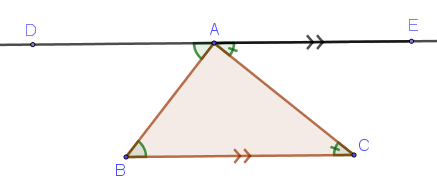
\includegraphics[width=0.5\textwidth]{proof_2}
\end{center}
두 엇각의 크기는 서로 같으므로
\begin{gather*}
\angle ABC=\fbox{(가)}\tag{1}\\
\angle ACB=\fbox{(나)}\tag{2}
\end{gather*}
따라서
\[\angle ABC+\angle BAC+\angle ACB\stackrel{(1), (2)}=\fbox{(가)}+\angle BAC+\fbox{(나)}=180^\circ\]
이다.
즉 삼각형의 세 각의 크기를 모두 더하면 \(180^\circ\)이다.
\qed
\end{mdframed}

%\newpage
예시 \ref{proof2})와 문제 \ref{proof3})
에서 사용한 증명방법을 \fbox{직접증명법}이라고 한다.
가정 \(p\)에서 출발하여 \(q\)에 도달시키면 명제 \(p\to q\)가 증명된다.

한 번에 결론으로 도달하지 못하고 여러 단계를 거쳐야 하는 경우도 있다.
이 때에는 \(p\to q\)이 참이고 \(q\to r\)가 참이면 \(p\to r\)가 참이라는, `삼단논법’에 의해 차근차근 단계를 밟아가면서 증명할 수 있다.

\bigskip
반면 \fbox{간접증명법}에는 \fbox{대우를 이용한 증명}과 \fbox{귀류법} 등이 있다.
\newpage

%
\subsection{대우를 이용한 증명}
명제 \(p\to q\)를 증명할 때, 주어진 명제를 증명하는 대신 대우를 증명하는 방법이다.
정리 \ref{pq9})에 따르면
대우 명제가 참이면 원래 명제도 참이므로, 대우만 증명해도 원래 명제가 참임을 알 수 있다.

%
\exam{\(n\)이 자연수일 때,}
\begin{quote}
\(n^2\)이 짝수이면 \(n\)도 짝수이다.
\end{quote}
가 참임을 증명하여라.
\begin{mdframed}\label{proof4}
이 명제의 대우인 `\(n\)이 홀수이면 \(n^2\)도 홀수이다.’가 참임을 보이면 된다.
\(n\)이 홀수이면 \(n=2k-1\)이다(단, \(k\)는 자연수).
그러면
\[n^2=(2k-1)^2=4k^2-4k+1=2(2k^2-2k)+1\]
이므로 \(n^2\)은 홀수이다.\qed
\end{mdframed}

%
\prob{\(n\)이 자연수일 때,}
\begin{quote}\label{proof5}
\(n^2\)이 \(3\)의 배수이면 \(n\)도 \(3\)의 배수이다
\end{quote}
가 참임을 증명하여라.
\bigskip\bigskip\bigskip
\newpage

%
\subsection{귀류법}
명제 \(p\to q\)를 증명할 때, 결론을 부정하여 가정과의 모순\footnotemark을 이끌어내어 증명하는 방법이다.
\footnotetext{\(p\to q\)꼴의 명제가 아닐 경우 이미 알려져 있는 사실과의 모순을 이끌어내도 된다.}

%명제 \(p\to q\)가 참이려면 \(P\subset Q\)가 성립해야 한다.
%즉 \(P-Q=\varnothing\), \(P\cap Q^c=\varnothing\)이 성립해야 한다.
%가정을 부정(\(Q^c\))하여 가정(\(P\))과의 모순(\(\varnothing\))을 이끌어내면, \(P\cap Q^c=\varnothing\)이 성립한다는 뜻이고 즉 \(P\subset Q\)가 성립한다는 뜻이므로 귀류법을 통해 명제를 증명할 수 있다.

결론을 부정(\(Q^c\))하여 가정(\(P\))과의 모순(\(\varnothing\))을 이끌어내면, \(P\cap Q^c=\varnothing\)이 성립한다는 뜻이다.
이것은 곧 \(P-Q=\varnothing\)이라는 말이고, 즉 \(P\subset Q\)가 성립한다는 뜻이다.
따라서 귀류법을 통해 명제 \(p\to q\)를 증명할 수 있다.

%
\exam{\(a\), \(b\), \(c\)가 정수일 때,}
\begin{quote}\label{proof6}
\(ax^2+bx+c=0\)이 정수인 근을 가지면 \(a\), \(b\), \(c\) 중 적어도 하나는 짝수이다.
\end{quote}
를 증명하여라.
\begin{mdframed}
결론을 부정하여 \(a\), \(b\), \(c\)가 모두 홀수라고 가정하자.
%이차방정식의 근이 정수이므로, 근은 짝수이거나 홀수이다.
\begin{itemize}
\item
만약 근이 짝수이면 \(ax^2\)은 짝수, \(bx\)는 짝수, \(c\)는 홀수이다.\\
그러면 \(ax^2+bx+c\)는 홀수가 되어 \(0\)이 될 수 없다.
\item
만약 근이 홀수이면 \(ax^2\)은 홀수, \(bx\)는 홀수, \(c\)는 홀수이다.\\
그러면 \(ax^2+bx+c\)는 홀수가 되어 \(0\)이 될 수 없다.
\end{itemize}
따라서  근은 짝수도 아니고 홀수도 아니다.
이것은 \(ax^2+bx+c=0\)이 정수인 근을 가진다는 가정에 모순이다.
%두 경우 모두 \(ax^2+bx+c\)은 홀수가 되어 \(0\)이 될 수 없으므로 모순이다.

따라서 \(a\), \(b\), \(c\) 중 적어도 하나는 짝수이다.
\qed
\end{mdframed}

\newpage
\begin{mdframed}
%
\defi{}
\begin{itemize}[leftmargin=*]\label{proof7}
\item
원이란, 평면 위의 한 점으로부터 일정한 거리에 있는 점들의 모임이다.
\item
원의 접선이란, 원과 한 점에서 만나는 직선을 말한다.
\end{itemize}
\end{mdframed}

%
\prob{다음은}
\begin{quote}\label{proof8}
원의 접선은 접선에서 그은 반지름과 수직이다.
\end{quote}
를 증명하는 과정이다.
(가), (나)에 알맞은 것을 채워 넣어라.
\begin{mdframed}[nobreak=false]
아래 그림과 같이 원 \(O\)와 직선 \(l\)이 \(T\)에서 접한다고 하자.
\begin{center}
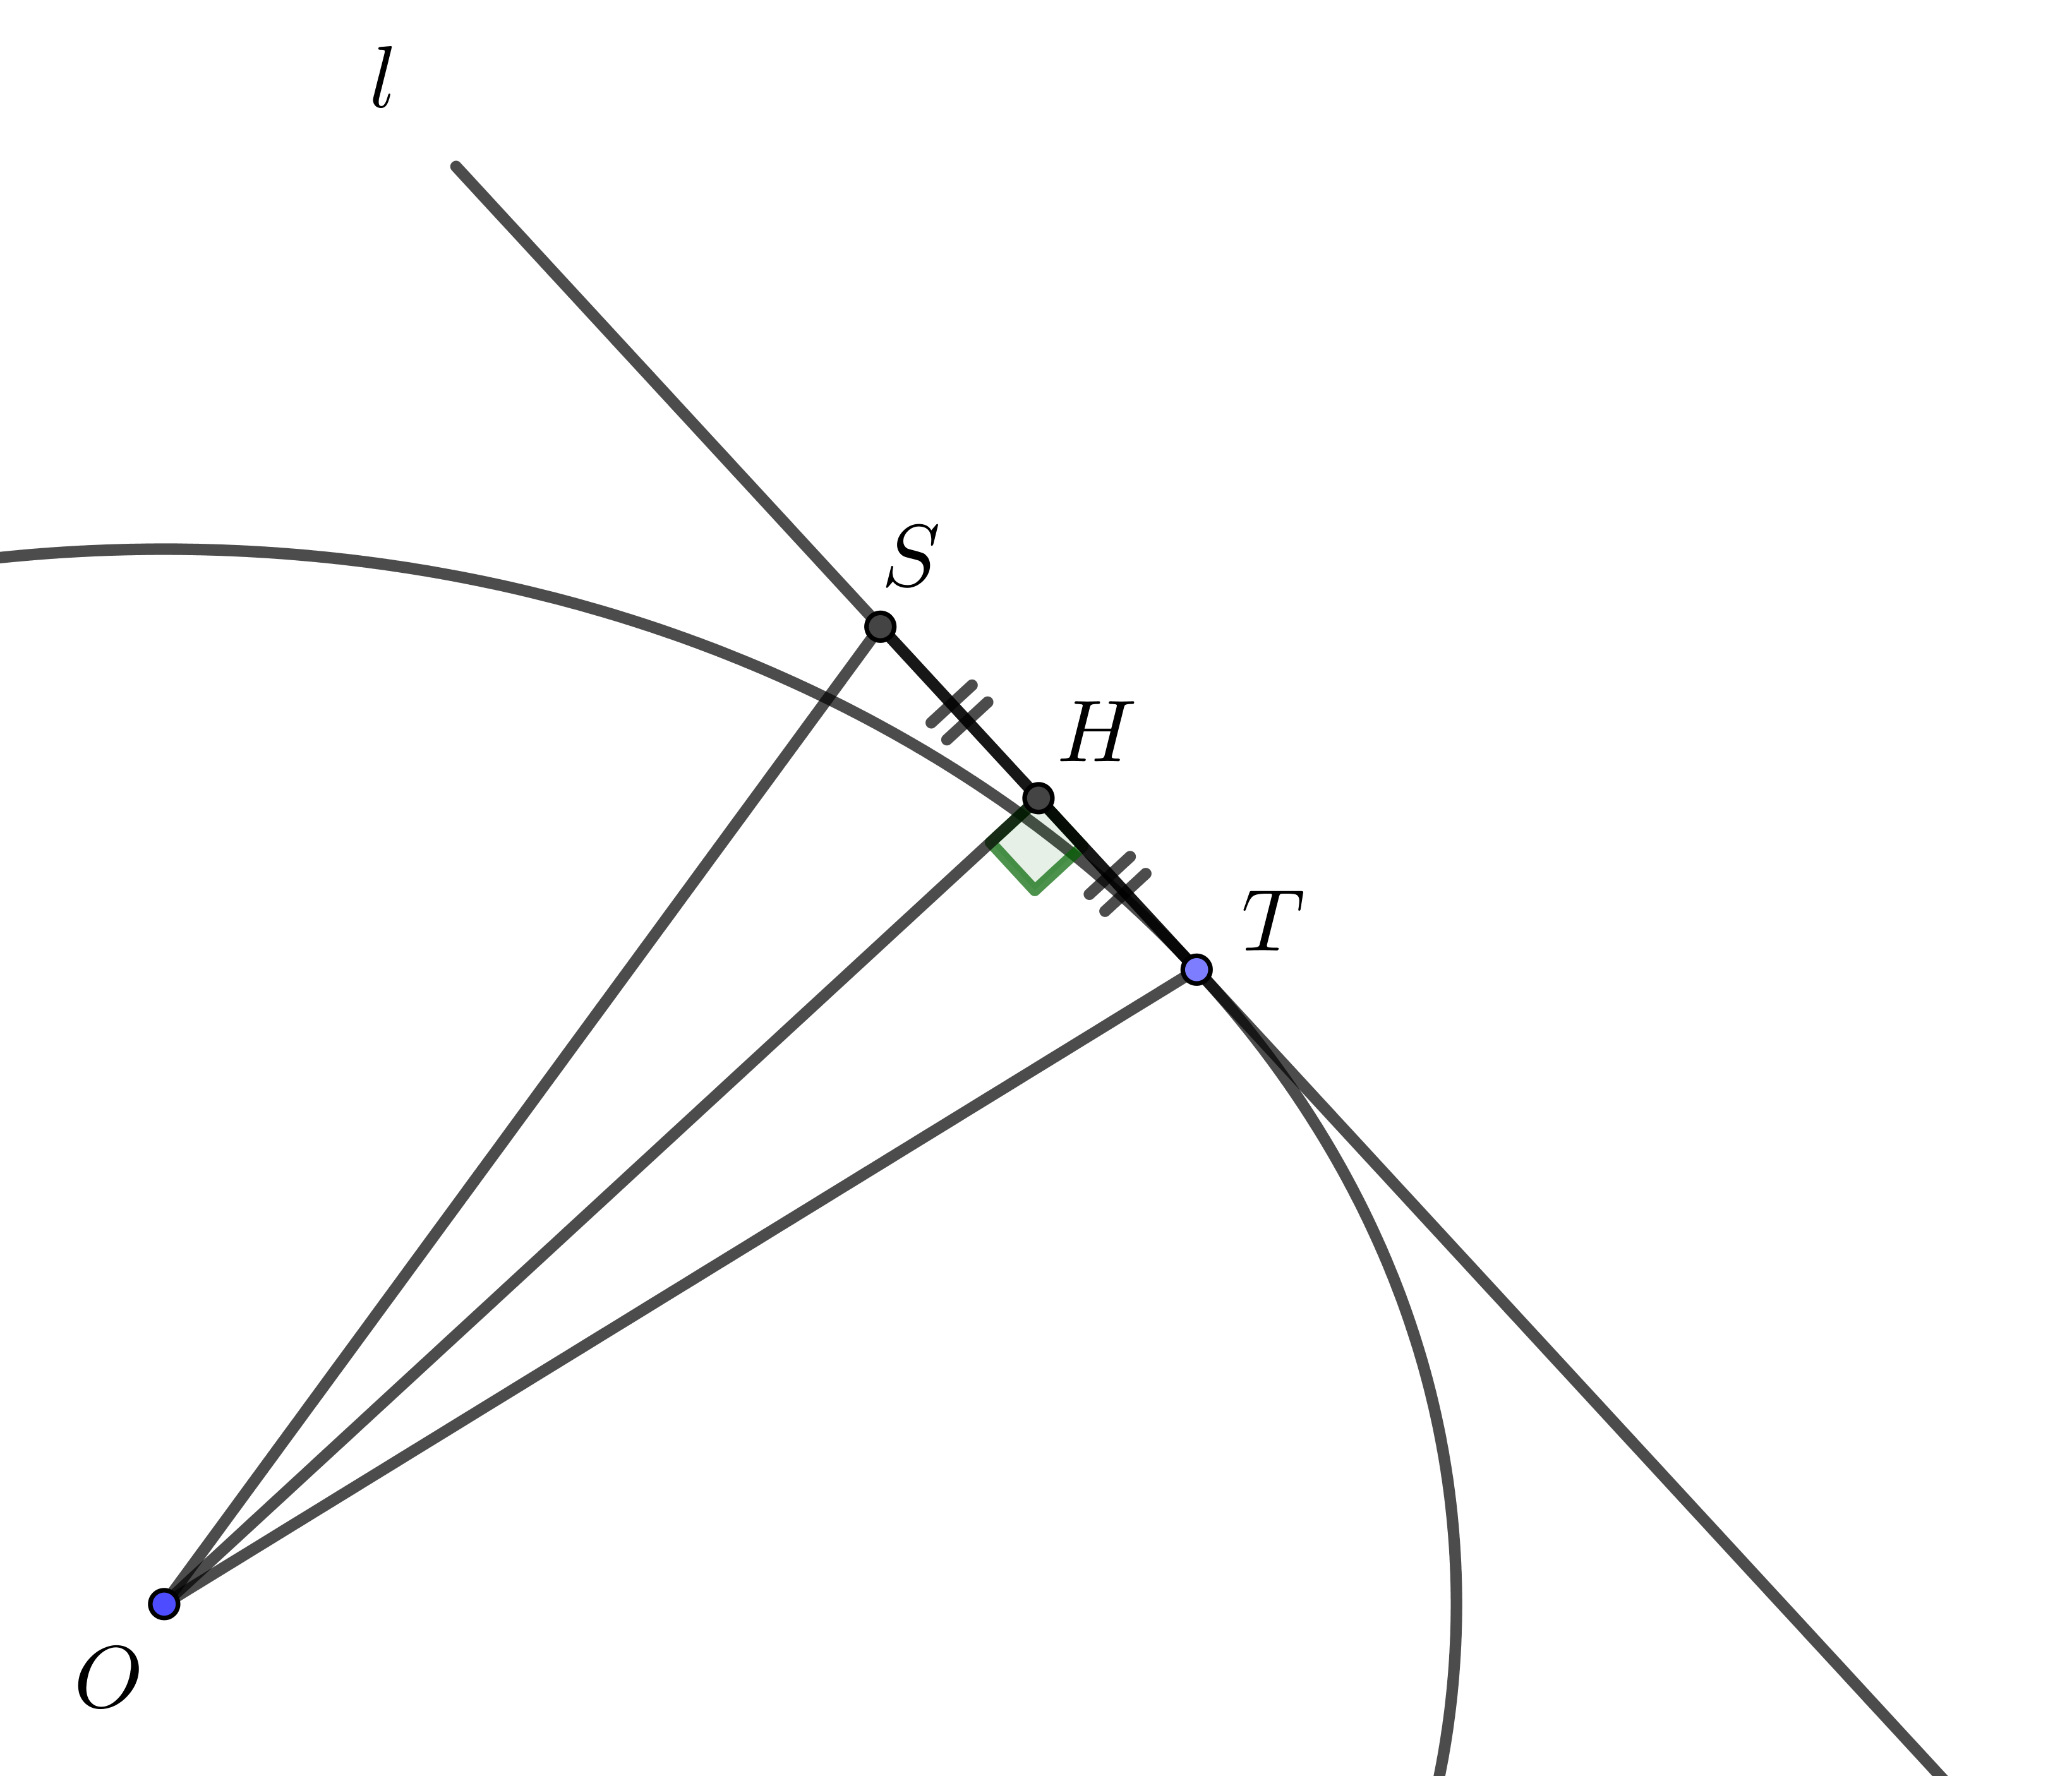
\includegraphics[width=0.5\textwidth]{proof_8}
\end{center}
주어진 명제를 부정하여 접선 \(l\)과 반지름 \(\ov OT\)가 수직하지 않는다고 가정하자.
원의 중심 \(O\)에서 직선 \(l\)에 내린 수선의 발을 \(H\)라고 하면 \(H\neq T\)이다.
\(T\)의 반대편에 \(\ov TH=\ov SH\)를 만족시키는 점 \(S\)를 직선 \(l\) 위에 잡으면,\\
\(\ov OH\)는 공통, \(\angle OHT=\angle OHS\), \(\ov TH=\ov SH\)로부터
\[\triangle OTH\equiv\fbox{\;\;(가)\;\;}(SAS)\]
이다.
따라서 \(\ov OT=\fbox{(나)}\)이다.
이것은 \(S\)가 원 \(O\) 위의 점이라는 뜻이며 \(S\)가 원 \(O\)와 직선 \(l\)의 교점이라는 뜻이다.
즉, 원 \(O\)와 직선 \(l\)은 두 개의 교점 \(T\), \(S\)을 가지게 되므로, 직선 \(l\)이 접선이라는 사실에 모순이다.

따라서 접선 \(l\)과 반지름 \(\ov OT\)는 수직하다.
\qed
\end{mdframed}


%%
\section{부등식의 증명}

%
\subsection{산술-기하 부등식}

%
\exam{}
\begin{enumerate}\label{ineq1}
\item
\(2\)와 \(8\)의 평균은 무엇일까?
보통은 \(\frac{2+8}2=5\)로 계산하여 \(5\)가 평균이라고 말한다.
이 평균을 \fbox{산술평균}이라고 부른다.
\item
한편, \(2=2^1\), \(2=2^3\)으로 생각하면, \(2\)와 \(8\)의 평균으로 \(2^2=4\)를 말할 수도 있다.
이 평균은 \fbox{기하평균}이라고 부른다.
\item
마지막으로 두 수의 역수인 \(\frac12\)와 \(\frac18\)의 평균이 어떤 수의 역수인지 생각해 볼수도 있다.
\[\frac{\frac12+\frac18}2=\frac1h\]
으로부터
\(h=\frac{16}5\)이다.
이 평균을 \fbox{조화평균}이라고 부른다.
\end{enumerate}

%
\prob{\(2\)와 \(18\)의 산술평균, 기하평균, 조화평균을 구하여라.}\label{ineq2}

\bigskip
\bigskip
\bigskip
\bigskip
\bigskip

\begin{mdframed}
%
\defi{산술평균, 기하평균, 조화평균}\label{ineq3}
\(a>0\), \(b>0\)일 때,\\
\(\frac{a+b}2\)를 산술평균, \(\sqrt{ab}\)를 기하평균, \(\frac{2ab}{a+b}\)를 조화평균이라고 한다.\footnotemark
\end{mdframed}
\footnotetext{
세 양수 \(a\), \(b\), \(c\)에 대하여,
\(\frac{a+b+c}3\)를 산술평균, \(\sqrt[3]{abc}\)를 기하평균, \(\frac{3abc}{ab+bc+ca}\)를 조화평균이라고 한다.
}

\newpage
예시 \ref{ineq1})에서 평균들의 대소관계를 비교해보면 산술평균(\(5\))이 제일 크고, 기하평균(\(4\))이 중간이며, 조화평균(\(\frac{16}5\))이 가장 작다.
일반적으로도 다음 관계가 성립한다.
\begin{mdframed}
%
\theo{\(a>0\), \(b>0\)일 때,\footnotemark}\label{ineq4}
\[\frac{a+b}2\ge\sqrt{ab}\ge\frac{2ab}{a+b}\quad(\text{단, 등호는 \(a=b\)일때 성립})\]
\end{mdframed}
\footnotetext{세 양수 \(a\), \(b\), \(c\)에 대하여
\[\frac{a+b+c}3\ge\sqrt[3]{abc}\ge\frac{3abc}{ab+bc+ca}\quad(\text{단, 등호는 \(a=b=c\)일때 성립})\]
}
\proo{}
\(\frac{a+b}2\ge\sqrt{ab}\iff a+b\ge2\sqrt{ab}\)이므로 \(a+b\ge2\sqrt{ab}\)를 증명해도 된다.
\[(a+b)^2-\left(2\sqrt{ab}\right)^2=(a^2+2ab+b^2)-4ab=(a-b)^2\ge0\]
이므로 증명되었다.
(단, 등호는 \(a=b\)일때 성립한다.)
%따라서 \(\frac{a+b}2\ge\sqrt{ab}\)이다.(단, 등호는 \(a=b\)일때 성립한다.)
\[\sqrt{ab}\ge\frac{2ab}{a+b}\iff(a+b)\sqrt{ab}\ge2ab\iff a+b\ge2\sqrt{ab}\]
에서 마지막 식을 증명하였으므로 \(\sqrt{ab}\ge\frac{2ab}{a+b}\)도 증명한 셈이 된다.
\qed

\bigskip\bigskip
정리 \ref{ineq4})을 조금 변형한 \(a+b\ge2\sqrt{ab}\)는 자주 쓰이는 중요한 부등식이다.

\begin{mdframed}
%
\theo{산술--기하 부등식}\label{ineq5}
\(a>0\), \(b>0\)일 때,
\[a+b\ge2\sqrt{ab}\]이다.
(단, 등호는 \(a=b\)일 때, 성립)
\end{mdframed}

%%
%\exam{}
%더해서 \(10\)이 되는 두 실수의 곱의 최댓값을 구하여라.

%\bigskip\bigskip\bigskip
\newpage
%
\subsection{코시--슈바르츠 부등식}
\begin{mdframed}
%
\theo{코시--슈바르츠 부등식\footnotemark}\label{ineq6}
\(a\), \(b\), \(x\), \(y\)가 모두 실수일 때,
\[(a^2+b^2)(x^2+y^2)\ge(ax+by)^2\]이다.
(단, 등호는 \(a:b=x:y\)일 때, 성립)
\end{mdframed}
\footnotetext{
\(a\), \(b\), \(c\), \(x\), \(y\), \(z\)가 모두 실수일 때,
\[(a^2+b^2+c^2)(x^2+y^2+z^2)\ge(ax+by+cz)^2\]이다.
(단, 등호는 \(a:b:c=x:y:z\)일 때, 성립)}
\proo{}
\begin{align*}
&(a^2+b^2)(x^2+y^2)-(ax+by)^2\\
=&(a^2x^2+a^2y^2+b^2x^2+b^2y^2)-(a^2x^2+2abxy+b^2y^2)\\
=&a^2y^2-2abxy+b^2x^2\\
=&(ay-bx)^2\ge0\quad
\end{align*}
(단, 등호는 \(ay=bx\)일 때, 즉 \(a:b=x:y\)일 때 성립)
\qed

%%
\section*{답}
\addcontentsline{toc}{chapter}{\protect\numberline{*}답}
\begin{multicols*}{2}
%
\ann{proposition2}{\(9\)}
$\begin{tabu}{c|ccc}
		&명제	&참/거짓	&조건	\\\hline
p_1		&\bigcirc	&거짓	&\\
p_2		&		&		&\\
p_3		&\bigcirc	&참		&\\
p_4		&\bigcirc	&거짓	&\\
p_5		&\bigcirc	&참		&\\
p_6		&		&		&\bigcirc\\
p_7		&\bigcirc	&참		&\\
\end{tabu}$
\par\bigskip\noindent
\(a=5\), \(c=3\), \(c=1\).
\(\therefore a+b+c=9\)

%
\an{proposition3}
%$\!$
\vspace{-10pt}\par\noindent
%\begin{quote}
\(P=\{4,8,12,\cdots\}\)\\
\(Q=\{0,2,4\}\)\\
\(R=\{2\}\)\\
\(S=U\)
%\end{quote}

%
\ann{negation7}\five
\one : `삼각형 \(ABC\)는 예각삼각형이 아니다.’\\
\two: `\(x\)는 \(9\)의 약수가 아니다.’\par\noindent
\three: `\(x\ge3\)’\\
\four: `\(x\neq1\) 이고 \(x\neq3\)이다.’\\

%
\an{negation8}
\begin{enumerate}
\item
\(\sqrt{25}\)는 무리수가 아니다.(참)
\item
\(11\)은 짝수도 아니고 \(3\)의 배수도 아니다.(참)
\end{enumerate}

%
\ann{negation9}{\(Q\subset P\)}
%\(P=\{2,3,4,5\}\), \(Q=\{2\}\)

%
\ann{negation10}{\(x\le2\) 또는 \(x\ge5\)}

%
\an{negation12}
\begin{enumerate*}[itemjoin={\:\:\:}]
\item참
\item거짓
\item거짓
\item참
\end{enumerate*}

%
\an{negation13}
\begin{enumerate*}[itemjoin={\:\:\:}]
\item거짓
\item참
\item참
\item참
\end{enumerate*}

%
\par\bigskip\noindent\textbf{예시 \ref{negation14})}\par\noindent
\begin{center}
\begin{tabu}[tabulinesep=100pt]{c|cccc}
	&\(p\)	&\(q\)	&\(r\)	&\(s\)\\\hline
③	&거짓	&참		&거짓	&참	\\
④	&거짓	&참		&거짓	&참	\\
⑤	&거짓	&참		&거짓	&참	\\
⑥	&거짓	&참		&거짓	&참	\\
⑦	&거짓	&참		&거짓	&참	\\
⑧	&거짓	&거짓	&참		&참	
\end{tabu}
\end{center}

%
\an{negation16}
\begin{enumerate}
\item
어떤 실수 \(x\)에 대하여 \(x^2\le0\)이다.
(참)
\item
모든 실수 \(x\)에 대하여 \(x^2=10\)이다.
(거짓)
\end{enumerate}

%
\an{pq4}
\begin{enumerate}%[itemjoin=\:\:]
\item
참
\item
거짓
\end{enumerate}
\begin{center}
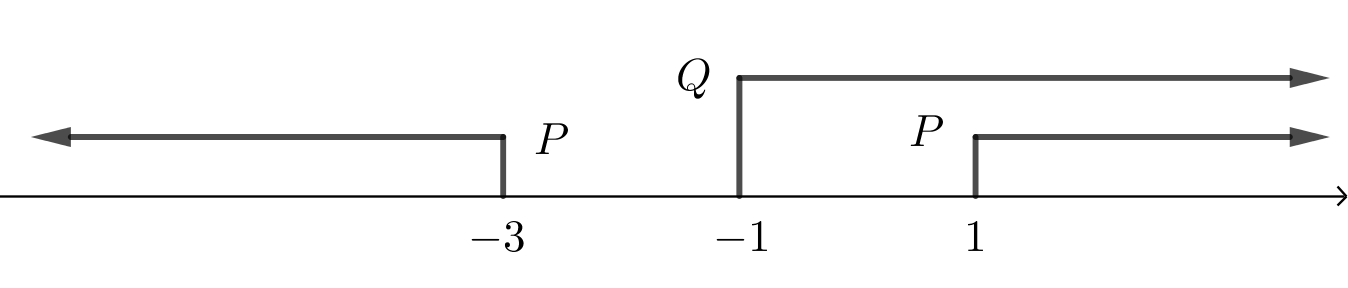
\includegraphics[width=0.45\textwidth]{pq_4}
\end{center}

%
\ann{pq5}\four

%
\an{pq8}
\begin{enumerate}
\item
역 : \parbox[t]{0.35\textwidth}{\(x=2\)이면 \(x^2-2x=0\)이다.(참)}\\
대우 :  \parbox[t]{0.32\textwidth}{\(x\neq2\)이면 \(x^2-2x\neq0\)이다.(거짓)}
\item
역 : \parbox[t]{0.35\textwidth}{\(-4< x<4\)이면 \(x^2<16\)이다.(참)}\\
대우 :  \parbox[t]{0.32\textwidth}{\(x\le-4\)이거나 \(x\ge4\)이면 \(x^2\ge16\)이다.(참)}
\end{enumerate}

%
\an{proof1}
\begin{enumerate}
\item정의
\item정리
\item정의
\item정리
\end{enumerate}

%
\an{proof3}
(가)\::\:\(\angle BAD\),\quad (나)\::\:\(\angle CAE\)

%
\an{proof5}
이 명제의 대우인 `\(n\)이 \(3\)의 배수가 아니면 \(n^2\)도 \(3\)의 배수가 아니다.’가 참임을 보이면 된다.
\(n\)이 \(3\)의 배수가 아니면 \(n\)은 \(3k-2\)꼴이거나 \(3k-1\)꼴이다(단, \(k\)는 자연수).
\begin{itemize}
\item
\(n=3k-2\)이면 
\begin{align*}
n^2
&=(3k-2)^2=9k^2-12k+4\\
&=3(3k^2-4k+1)+1
\end{align*}
\item
\(n=3k-1\)이면 
\begin{align*}
n^2
&=(3k-1)^2=9k^2-6k+1\\
&=3(3k^2-2k)+1
\end{align*}
\end{itemize}
이다. 두 경우 모두 \(n^2\)은 \(3\)의 배수가 아니다.
\qed

%
\an{proof8}
(가)\::\:\(\triangle OSH\),\quad (나)\::\:\(\ov OS\)

%
\an{ineq2}
\begin{itemize}
\item
산술평균 : \(10\)
\item
기하평균 : \(6\)
\item
조화평균 : \(\frac{18}5\)
\end{itemize}
\end{multicols*}

%%
\section*{요약}
\addcontentsline{toc}{chapter}{\protect\numberline{*}요약}
\begin{enumerate}[label=\arabic*.,itemsep=15pt]
\item
명제와 조건, 진리집합
\begin{itemize}
\item
\(3\)은 \(6\)의 약수이다. \(\cdots\cdots\cdots\) 명제(참)
\item
\(4\)는 \(6\)의 약수이다. \(\cdots\cdots\cdots\) 명제(거짓)
\item
\(x\)는 \(6\)의 약수이다. \(\cdots\cdots\cdots\) 조건\\
\(\Rightarrow\text{진리집합}=\{1,2,3,6\}\) 
\end{itemize}
\item
부정
\begin{itemize}
\item
\(\sim(p\text{ 또는 }q)\iff\sim p\text{ 그리고 }\sim q\)
\item
\(\sim(p\text{ 그리고 }q)\iff\sim p\text{ 또는 }\sim q\)
\item
\(\sim\left(\text{모든 \(x\)에 대하여 \(p(x)\)이다.}\right)\iff\text{어떤 \(x\)에 대하여 \(\sim p(x)\)이다.}\)
\item
\(\sim\left(\text{어떤 \(x\)에 대하여 \(p(x)\)이다.}\right)\iff\text{모든 \(x\)에 대하여 \(\sim p(x)\)이다.}\)
\end{itemize}
\item
\(p\to q\)꼴의 명제
\begin{itemize}
\item
\(P\subset Q\)이면 \(p\to q\)가 참이다(\(p\Longrightarrow q\)).\\
\(P\not\subset Q\)이면 \(p\to q\)가 거짓이다(\(p\not\Longrightarrow q\)).
\item
역 : \(q\to p\),\qquad 대우 : \(\sim q\to\sim p\)
\item
\(p\Longrightarrow q\)이면
\(p\)는 \(q\)이기 위한 충분조건,
\(q\)는 \(p\)이기 위한 필요조건
\item
\(p\iff q\)이면
\(p\)는 \(q\)이기 위한 필요충분조건
\end{itemize}
\item
정의, 정리, 증명
\begin{itemize}
\item
직접증명법 -- 삼단논법
\item
간접증명법 -- 대우를 이용한 증명, 귀류법
\end{itemize}
\item
부등식의 증명
\begin{itemize}
\item
산술--기하 부등식 :
\(a+b\ge2\sqrt{ab}\)\\
(단, 등호는 \(a=b\)일 때 성립)
\item
코시--슈바르츠 부등식 :
\((a^2+b^2)(x^2+y^2)\ge(ax+by)^2\)\\
(단, 등호는 \(a:b=x:y\)일 때 성립)
\end{itemize}
\end{enumerate}
\end{document}